\documentclass[conference]{IEEEtran}

\usepackage[T1]{fontenc}
\usepackage[utf8]{inputenc}
\usepackage{cite}
\usepackage{amsmath,amssymb}
\usepackage{graphicx}
\usepackage{textcomp}
\usepackage{booktabs}
\usepackage{array}
\usepackage{url}
\usepackage[caption=false,font=footnotesize]{subfig}
\usepackage{balance}

% =========================================================
% RISULTATI SPERIMENTALI
% I valori seguenti corrispondono alle run rappresentative definitive
% selezionate per il report; ciascuna misura ha numerosita n=1.
% =========================================================
\newcommand{\AvgConvTime}{2.010}
\newcommand{\SumConvTime}{1.069}
\newcommand{\MinConvTime}{2.008}
\newcommand{\MaxConvTime}{1.054}

\newcommand{\TCLocalFirstConv}{4}
\newcommand{\TCLocalStable}{9}
\newcommand{\TCAWSFirstConv}{2}
\newcommand{\TCAWSStable}{10}

\begin{document}

\title{Gossip-Based Distributed Data Aggregation}

\author{
\IEEEauthorblockN{Luca Capone}
\IEEEauthorblockA{
Dipartimento di Ingegneria Informatica\\
Università degli Studi di Roma Tor Vergata\\
Roma, Italia
}
}

\maketitle

\begin{abstract}
Questo lavoro presenta la progettazione, l'implementazione e la valutazione di un servizio decentralizzato per l'aggregazione distribuita dei dati basato su protocollo gossip. Il sistema, sviluppato individualmente in Go, non utilizza un coordinatore centrale per il calcolo: ogni nodo mantiene una vista locale della membership e dei contributi, scambia periodicamente stato tramite UDP e applica merge deterministici e idempotenti. Sono supportate somma, media, minimo e massimo. La soluzione comprende failure detection per crash fail-stop, leave, restart/rejoin, versionamento durevole e osservabilità. La valutazione combina test unitari, concorrenti, in-memory, su socket reali e Docker Compose a tre e sei nodi. Una modalità separata basata su Linux Traffic Control e NetEm introduce delay e jitter artificiali, mentre il deployment cloud utilizza Docker Compose su una singola istanza AWS EC2. Nelle esecuzioni osservate, i sei nodi convergono agli oracle configurati; i test verificano inoltre continuità dei peer superstiti e riconvergenza negli scenari di failure e recovery considerati.
\end{abstract}

\begin{IEEEkeywords}
sistemi distribuiti, gossip protocol, aggregazione distribuita, convergenza eventuale, fault tolerance, membership, Docker Compose, AWS EC2, Traffic Control
\end{IEEEkeywords}

% =========================================================
\section{Introduzione}
% =========================================================

L'aggregazione di informazioni prodotte da molteplici nodi è un problema ricorrente nei sistemi distribuiti. Operazioni quali somma, media, minimo e massimo sono semplici quando i dati sono raccolti da un singolo processo, ma diventano più complesse quando i contributi sono distribuiti tra nodi indipendenti, la comunicazione può essere ritardata o persa e i partecipanti possono entrare, uscire o fallire durante l'esecuzione.

Un approccio centralizzato, nel quale tutti i nodi inviano i propri valori a un coordinatore, semplifica il calcolo ma introduce un punto privilegiato dell'architettura e può rappresentare un limite per fault tolerance e scalabilità. I protocolli gossip adottano invece una strategia decentralizzata: i nodi scambiano periodicamente informazioni con un sottoinsieme di peer e propagano progressivamente lo stato nel sistema \cite{demers1987,jelasity2005}. Tali protocolli privilegiano disponibilità, semplicità e convergenza eventuale rispetto a proprietà di consistenza forte.

Questo progetto individuale realizza un servizio di \emph{gossip-based distributed data aggregation} in Go. Ogni nodo è equivalente agli altri e mantiene localmente sia i contributi necessari al calcolo dell'aggregato sia una vista della membership. I deployment forniti usano seed statici. Il nodo implementa anche il client di un contratto HTTP di join opzionale, verificato dai test ma non distribuito come servizio nel Compose; entrambi i meccanismi riguardano soltanto il bootstrap. Dopo l'avvio, aggregazione, disseminazione e failure detection procedono peer-to-peer.

Il sistema supporta quattro operazioni: \emph{sum}, \emph{average}, \emph{min} e \emph{max}. L'architettura integra inoltre deduplicazione dei messaggi, versionamento dello stato, gestione dei messaggi fuori ordine, stati di membership \texttt{alive}, \texttt{suspect}, \texttt{dead} e \texttt{leave}, nonché restart e rejoin della stessa identità logica.

La valutazione considera correttezza dell'aggregazione, convergenza, crash fail-stop, leave, restart/rejoin, recovery dopo una partizione temporanea e sensibilità a ritardi sintetici. Il sistema viene eseguito tramite Docker Compose sia localmente sia su una singola istanza AWS EC2. Una modalità sperimentale separata utilizza Linux \texttt{tc/netem} per introdurre delay e jitter senza modificare l'algoritmo applicativo.

Il codice sorgente e la documentazione tecnica del progetto sono disponibili nel repository GitHub del progetto.\footnote{\url{https://github.com/lucacapone/SDCC-project}}

% =========================================================
\section{Contesto e fondamenti}
% =========================================================

\subsection{Protocolli gossip}

I protocolli gossip costituiscono un paradigma di comunicazione decentralizzato ampiamente utilizzato nei sistemi distribuiti per disseminare stato e realizzare altre forme di coordinamento \cite{vansteen2023,kermarrec2007}. L'idea deriva dagli algoritmi epidemici utilizzati per la manutenzione di database replicati \cite{demers1987}. A ogni round un nodo seleziona uno o più peer, comunica parte del proprio stato e integra le informazioni ricevute.

Questo modello presenta proprietà utili nei sistemi distribuiti: non richiede una topologia rigida, tollera la perdita di singoli messaggi e consente alla conoscenza di propagarsi attraverso scambi successivi. Il prezzo da pagare è che i nodi possono mantenere temporaneamente viste differenti del sistema.

Il gossip può essere utilizzato direttamente anche per la computazione di informazioni aggregate. In letteratura sono state proposte tecniche per la computazione decentralizzata di somme, medie e altre funzioni globali \cite{kempe2003,jelasity2005}. Il presente lavoro segue la stessa filosofia generale, ma mantiene esplicitamente contributi versionati associati alle identità dei nodi, così da integrare il calcolo dell'aggregato con la membership dinamica.

\subsection{Convergenza eventuale}

Il sistema non tenta di garantire consistenza forte o linearizzabilità. L'obiettivo è la \emph{convergenza eventuale}: se la membership diventa stabile, non vengono introdotti nuovi contributi e i messaggi continuano a essere scambiati, i nodi devono convergere allo stesso insieme di informazioni e quindi allo stesso risultato aggregato.

Per ottenere questa proprietà, gli update sono associati a versioni e le operazioni di merge evitano regressioni quando arrivano messaggi duplicati o fuori ordine. Tale approccio presenta analogie con strutture dati convergenti e con i principi dei Conflict-Free Replicated Data Types \cite{shapiro2011}, pur non implementando un CRDT generico.

\subsection{Membership e failure detection}

In un ambiente distribuito l'aggregazione non può essere separata dalla conoscenza dei nodi attivi. Un valore appartenente a un nodo definitivamente non raggiungibile non deve continuare necessariamente a contribuire al risultato corrente.

Il sistema utilizza una membership locale con quattro stati: \texttt{alive}, \texttt{suspect}, \texttt{dead} e \texttt{leave}. I messaggi gossip ricevuti agiscono anche come heartbeat impliciti. La transizione verso \texttt{suspect} e successivamente \texttt{dead} è determinata da timeout. Il modello è concettualmente vicino ai protocolli di membership infection-style, come SWIM \cite{das2002}, pur adottando una propria implementazione e integrandola direttamente con lo stato aggregativo.

% =========================================================
\section{Progettazione della soluzione}
% =========================================================

\subsection{Obiettivi di progetto}

La soluzione è stata progettata perseguendo cinque obiettivi principali:

\begin{enumerate}
    \item eliminare un coordinatore centrale dal calcolo degli aggregati;
    \item garantire convergenza in presenza di messaggi duplicati o fuori ordine;
    \item continuare l'elaborazione quando uno o più nodi diventano indisponibili;
    \item consentire a un nodo riavviato di rientrare correttamente nel cluster;
    \item rendere configurabili i parametri di rete, gossip, membership e aggregazione.
\end{enumerate}

Tutti i nodi eseguono lo stesso processo Go e sono logicamente equivalenti. I seed influenzano soltanto il bootstrap e non introducono un nodo responsabile della computazione globale. L'endpoint di join è un'integrazione client opzionale; nessun servizio join centrale fa parte dei deployment forniti.

\begin{figure*}[t]
    \centering
    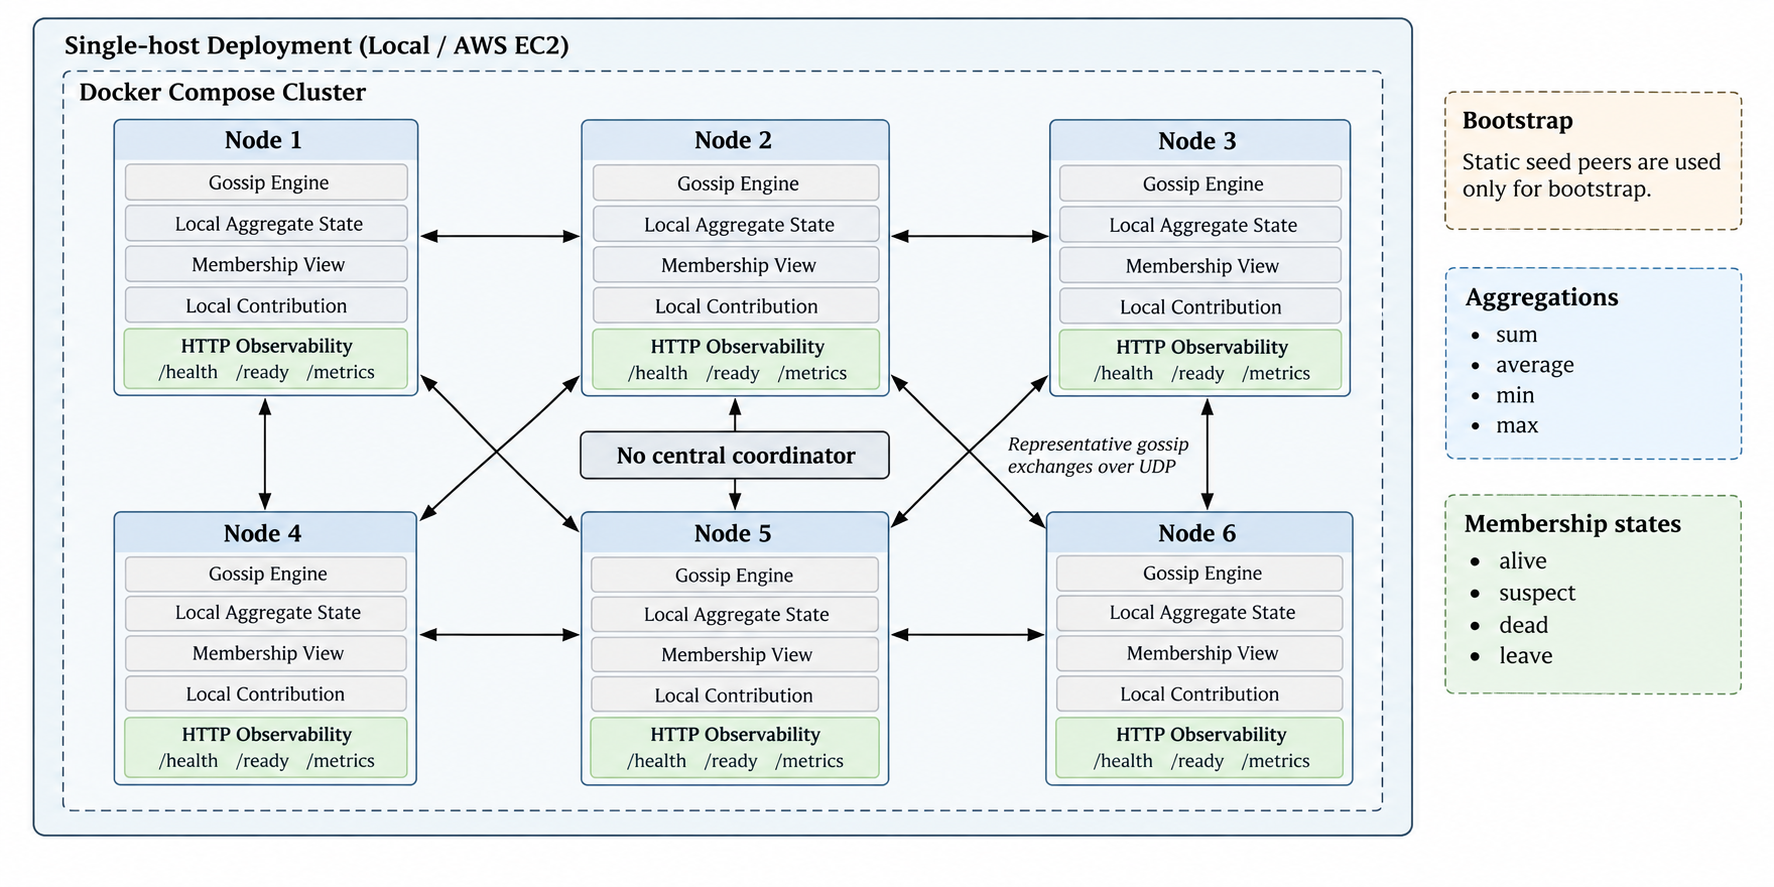
\includegraphics[width=0.94\textwidth]{figures/architecture.png}
    \caption{Architettura logica del sistema. Ogni nodo equivalente mantiene localmente stato aggregativo e membership, scambia messaggi gossip tramite UDP e pubblica endpoint HTTP di osservabilit\`a; i seed intervengono soltanto nel bootstrap.}
    \label{fig:architecture}
\end{figure*}

\subsection{Componenti di un nodo}

L'implementazione separa le responsabilità principali in moduli. Il package di configurazione gestisce default, file YAML/JSON, override tramite variabili di ambiente e validazione. Il modulo \emph{identity} assegna una generation persistente al processo. La membership conserva lo stato dei peer e applica timeout e transizioni. Il transport implementa la comunicazione UDP, mentre il gossip engine gestisce round, selezione dei peer, invio, ricezione e merge. Il package di aggregazione implementa le quattro operazioni supportate. Infine, il modulo di observability raccoglie metriche ed emette log strutturati.

Lo stato mutabile del gossip engine è sincronizzato per consentire al loop periodico dei round e al percorso di ricezione dei messaggi di operare in concorrenza.

\subsection{Stato locale e messaggi}

Ogni messaggio gossip contiene almeno l'identità dell'origine, un identificatore del messaggio, un timestamp, la versione del protocollo, una versione dello stato, lo stato aggregativo e un digest della membership.

La versione dello stato è rappresentata dalla coppia
\begin{equation}
V=(epoch,counter).
\end{equation}

L'\emph{epoch} deriva dalla generation persistente del processo e cambia a ogni nuovo avvio della stessa identità. Il \emph{counter} cresce invece durante la singola esecuzione.

L'identificatore del messaggio permette di rilevare consegne duplicate, mentre la versione permette di distinguere informazioni nuove da informazioni obsolete. Un contributo associato a uno specifico nodo viene sostituito soltanto da una versione più recente. Questa scelta evita che un datagramma ritardato possa riportare lo stato a una versione precedente.

\subsection{Protocollo di disseminazione}

Il protocollo implementato è di tipo \emph{push}. A ogni intervallo di gossip il nodo:

\begin{enumerate}
    \item aggiorna la membership applicando eventuali timeout;
    \item aggiorna il proprio contributo e ricalcola la stima;
    \item incrementa round e versione locale;
    \item esclude se stesso e i peer non eleggibili;
    \item ordina i peer disponibili;
    \item invia il proprio stato a un massimo di \texttt{fanout} peer.
\end{enumerate}

La selezione utilizza una finestra circolare deterministica. In una membership stabile con $N$ target, l'intero insieme dei peer viene visitato entro un massimo teorico di
\begin{equation}
\left\lceil\frac{N}{fanout}\right\rceil
\end{equation}
round.

Non viene effettuato un retry immediato del singolo datagramma UDP fallito. La ridondanza è ottenuta naturalmente attraverso i round successivi.

\subsection{Membership-aware aggregation}

Sia membership sia aggregazione partecipano al calcolo del risultato esposto. Indichiamo con $\mathcal{A}$ l'insieme delle identità considerate \texttt{alive} in un determinato nodo.

Per i valori locali $v_i$, la somma è
\begin{equation}
S=\sum_{i\in\mathcal{A}} v_i.
\end{equation}

La media è
\begin{equation}
\overline{x}=\frac{\sum_{i\in\mathcal{A}} v_i}{|\mathcal{A}|}.
\end{equation}

Minimo e massimo sono rispettivamente
\begin{equation}
m=\min_{i\in\mathcal{A}} v_i,
\qquad
M=\max_{i\in\mathcal{A}} v_i.
\end{equation}

Nell'implementazione della media ogni nodo conserva metadata di tipo somma/conteggio, mantenendo separato il contributo originario dalla stima corrente per evitare fenomeni di drift.

I contributi appartenenti a nodi \texttt{suspect}, \texttt{dead} o \texttt{leave} non partecipano al risultato visibile, ma possono essere conservati nei metadata. Questo consente di reagire alla failure detection senza distruggere informazioni potenzialmente utili in caso di rejoin.

% =========================================================
\section{Dettagli della soluzione}
% =========================================================

\subsection{Failure detection e rejoin}

Il parametro esterno \texttt{membership\_timeout\_ms}, indicato con $T_m$, determina $T_{suspect}=\max(1\text{ ms},T_m/2)$ e $T_{dead}=\max(T_{suspect}+1\text{ ms},T_m)$.

La configurazione viene rifiutata se la soglia di sospetto non è compatibile con il tempo necessario al gossip per coprire i peer configurati. Questo controllo riduce la probabilità di classificare erroneamente come non raggiungibile un nodo che semplicemente non è ancora stato contattato.

Quando un processo viene riavviato, mantiene la stessa \texttt{node\_id}, ma alloca una generation superiore a quella salvata nel proprio volume durevole. Tale valore è usato come incarnation della membership ed epoch dello stato, consentendo al nuovo processo di prevalere su informazioni o tombstone della precedente esecuzione. La rimozione del volume elimina questa continuità durevole.

\subsection{Configurazione}

Non vengono utilizzati parametri operativi hard-coded come unica modalità di configurazione. Il loader segue la precedenza
\begin{equation}
default \rightarrow file \rightarrow environment \rightarrow validation.
\end{equation}

Sono supportati file YAML e JSON. Tra i parametri configurabili figurano identità, indirizzo e porta del nodo, peer iniziali, intervallo gossip, fanout, timeout della membership, aggregazione, valore iniziale e livello di logging.

Nella configurazione a sei nodi utilizzata negli esperimenti, i valori iniziali sono
\begin{equation}
10,\;30,\;50,\;70,\;90,\;110.
\end{equation}

Gli oracle risultanti sono quindi
\begin{equation}
average=60,\quad sum=360,\quad min=10,\quad max=110.
\end{equation}

Le configurazioni correnti del cluster a sei nodi utilizzano un intervallo gossip di 1000 ms, fanout pari a 5 e membership timeout di 10000 ms. Poiché ogni nodo ha cinque peer, in questo specifico scenario il fanout consente di contattare tutti gli altri partecipanti nello stesso round.

\subsection{Transport e osservabilità}

La comunicazione gossip utilizza UDP. Il transport mantiene un socket persistente e tratta il payload serializzato come una sequenza di byte senza interpretarne il contenuto.

UDP non garantisce consegna né ordinamento. Il sistema non tenta quindi di ottenere affidabilità dal livello di trasporto, ma utilizza versionamento, deduplicazione e ripetizione dei round gossip per tollerare perdite o riordinamenti.

Ogni processo espone inoltre un server HTTP dedicato all'osservabilità, separato dal traffico gossip. Gli endpoint principali sono:

\begin{itemize}
    \item \texttt{/health}, per la liveness del processo;
    \item \texttt{/ready}, per verificare che bootstrap ed engine siano stati avviati;
    \item \texttt{/metrics}, con metriche in formato compatibile con Prometheus.
\end{itemize}

Le metriche includono numero di round, merge remoti, peer conosciuti, stima corrente, uptime, readiness e stato del lifecycle.

La readiness non coincide con la convergenza: un nodo può essere completamente avviato ma non aver ancora ricevuto tutte le informazioni necessarie per il valore globale corretto.

\subsection{Deployment e testing}

L'immagine applicativa viene costruita tramite Docker con una fase di build Go 1.22 e una runtime image minimale non-root. Docker Compose viene utilizzato per avviare sia il cluster canonico a tre nodi sia la configurazione scale a sei nodi \cite{dockercompose}.

Il deployment cloud utilizza una singola istanza AWS EC2 \cite{awsec2}. I sei nodi sono processi containerizzati indipendenti sulla stessa macchina virtuale e comunicano attraverso una rete bridge Docker. Le porte gossip e observability non devono essere esposte pubblicamente.

La strategia di testing, riassunta nella Tabella~\ref{tab:testing}, separa le proprietà algoritmiche dalle prove sul deployment effettivo. I test di partizione verificano continuità durante l'isolamento temporaneo, recovery e riconvergenza finale, senza caratterizzare completamente le stime nelle due componenti durante l'intera partizione.

\begin{table}[t]
\centering
\caption{Livelli della strategia di testing}
\label{tab:testing}
\scriptsize
\begin{tabular}{@{}p{0.18\columnwidth}p{0.48\columnwidth}p{0.22\columnwidth}@{}}
\toprule
\textbf{Livello} & \textbf{Proprietà principali} & \textbf{Ambiente} \\
\midrule
Unità/contratto & Configurazione, aggregazioni, membership, generation, gossip e osservabilità & Go, deterministico \\
Concorrenza & Accessi concorrenti a membership, round/ricezione e allocazione generation & Go race detector \\
Transport & Contratto del transport e ciclo start/send/close & Socket UDP reali \\
Integrazione & Convergenza, duplicati/out-of-order, leave e rejoin & Cluster in-memory \\
Deployment & Convergenza a 3/6 nodi, crash/restart e partizione temporanea & Docker Compose \\
Pipeline & Oracle, completezza dei nodi, tolleranza, CSV e SVG & Log osservativi \\
\bottomrule
\end{tabular}
\end{table}

La pipeline di misura emette eventi strutturati \texttt{convergence\_sample}. Uno strumento separato raccoglie i log, ricostruisce le serie temporali e genera CSV e grafici SVG. La convergenza viene definita come il primo istante dal quale tutte le serie dei nodi rimangono entro una tolleranza assoluta di 0.05 rispetto all'oracle fino alla fine della finestra osservata; la readiness HTTP non fa parte di questo criterio.

% =========================================================
\section{Risultati}
% =========================================================

\subsection{Configurazione sperimentale}

La valutazione principale è stata effettuata sul cluster a sei nodi, considerato lo scenario più rappresentativo tra quelli inclusi nel progetto. Tutti i nodi utilizzano la stessa operazione di aggregazione durante una singola esecuzione. I valori temporali riportati sono i risultati definitivi delle run selezionate, una singola run rappresentativa per aggregazione ($n=1$): sono misure descrittive, non medie statistiche, bound o prestazioni garantite.

La Tabella~\ref{tab:setup} riassume la configurazione principale.

\begin{table}[t]
\centering
\caption{Configurazione del cluster sperimentale}
\label{tab:setup}
\footnotesize
\begin{tabular}{@{}ll@{}}
\toprule
\textbf{Parametro} & \textbf{Valore} \\
\midrule
Nodi & 6 \\
Valori & 10, 30, 50, 70, 90, 110 \\
Transport & UDP \\
Gossip interval & 1000 ms \\
Fanout & 5 \\
Membership timeout & 10000 ms \\
Deployment & Docker Compose \\
Aggregazioni & sum, average, min, max \\
\bottomrule
\end{tabular}
\end{table}

\subsection{Convergenza delle aggregazioni}

Per ciascuna operazione il cluster è stato avviato con gli stessi sei contributi. Le serie temporali sono state ricostruite dai campioni generati dai nodi e confrontate con l'oracle calcolato a partire dalle configurazioni.

Nelle run baseline selezionate, tutte e quattro le aggregazioni hanno raggiunto il risultato atteso con tutti i sei nodi osservati. La Tabella~\ref{tab:convergence} riporta il primo istante dal quale tutte le serie restano entro la tolleranza assoluta 0.05 fino alla fine della finestra osservata.

\begin{table}[t]
\centering
\caption{Convergenza nel cluster a sei nodi}
\label{tab:convergence}
\scriptsize
\setlength{\tabcolsep}{3pt}
\begin{tabular}{@{}lrrrr@{}}
\toprule
\textbf{Aggregazione} & \textbf{Oracle} & \textbf{Tempo [s]} & \textbf{Campioni} & \textbf{Nodi} \\
\midrule
Average & 60  & \AvgConvTime & 152 & 6/6 \\
Sum     & 360 & \SumConvTime & 153 & 6/6 \\
Min     & 10  & \MinConvTime & 134 & 6/6 \\
Max     & 110 & \MaxConvTime & 138 & 6/6 \\
\bottomrule
\end{tabular}
\end{table}

In particolare, le run definitive selezionate hanno raggiunto il criterio della pipeline a \AvgConvTime~s per la media, \SumConvTime~s per la somma, \MinConvTime~s per il minimo e \MaxConvTime~s per il massimo. Ogni valore deriva da una sola esecuzione e non costituisce una media statistica o un benchmark prestazionale generale.

\begin{figure*}[t]
    \centering
    \subfloat[Average]{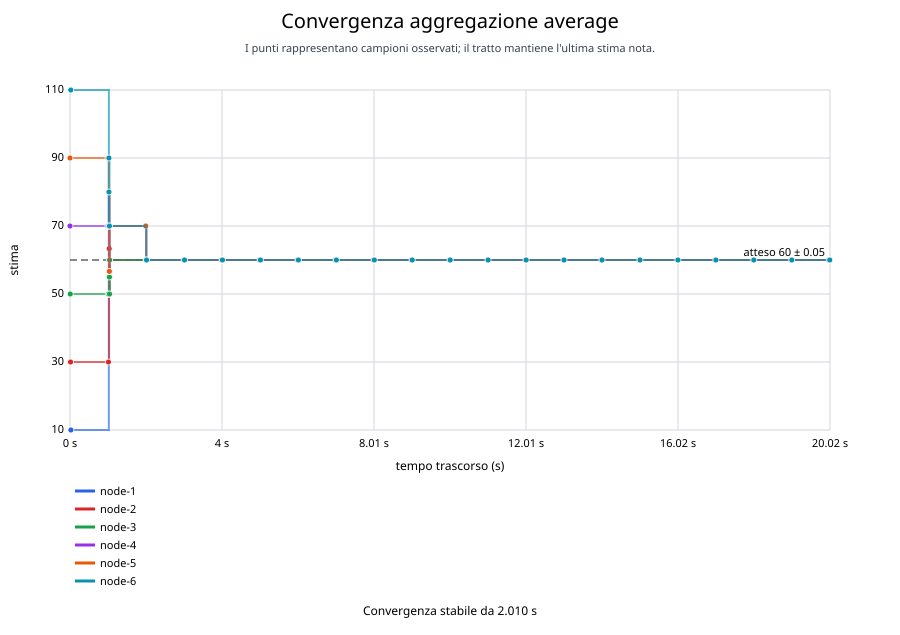
\includegraphics[width=0.48\textwidth]{figures/convergence_average_6nodes.png}}\hfill
    \subfloat[Sum]{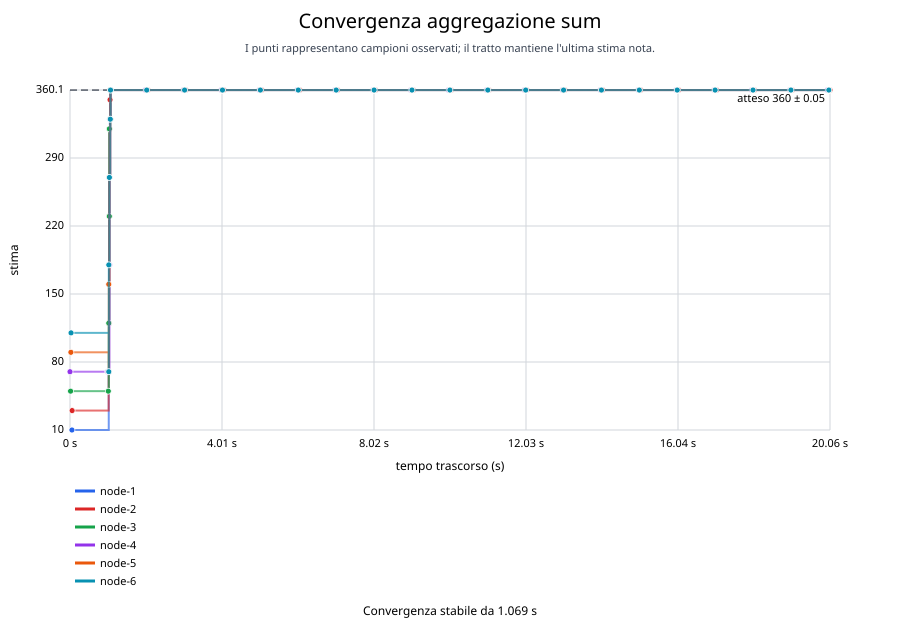
\includegraphics[width=0.48\textwidth]{figures/convergence_sum_6nodes.png}}\\
    \subfloat[Min]{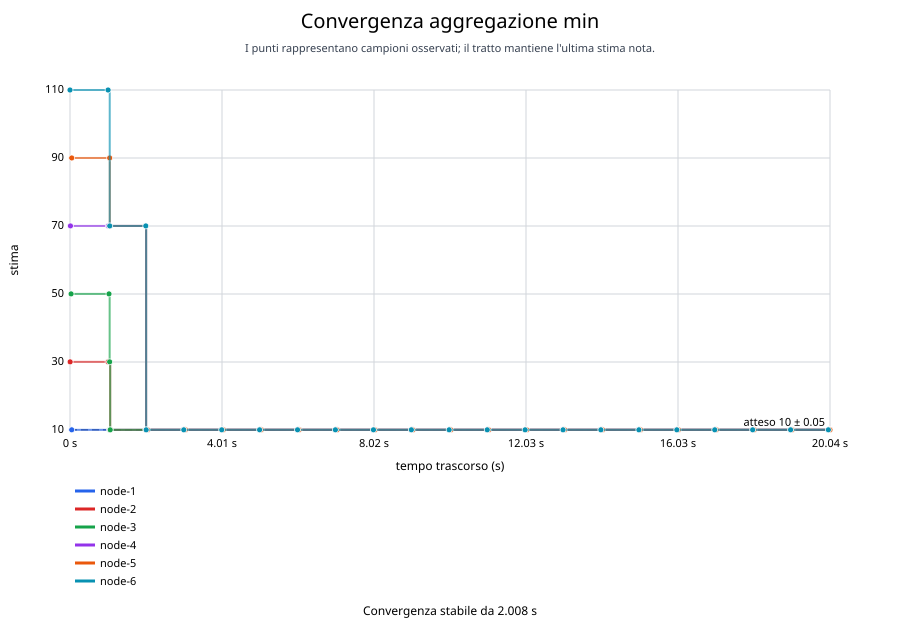
\includegraphics[width=0.48\textwidth]{figures/convergence_min_6nodes.png}}\hfill
    \subfloat[Max]{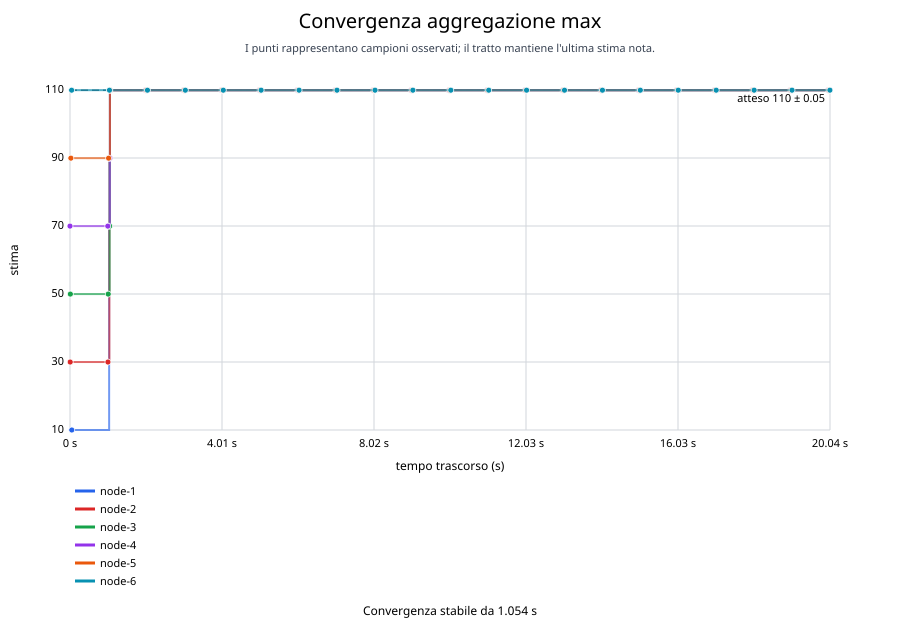
\includegraphics[width=0.48\textwidth]{figures/convergence_max_6nodes.png}}
    \caption{Serie di convergenza baseline, senza delay NetEm, per le quattro aggregazioni sul cluster a sei nodi. Le linee di riferimento rappresentano gli oracle configurati.}
    \label{fig:convergence-aggregations}
\end{figure*}

Questi risultati verificano non soltanto che i nodi raggiungano lo stesso valore, ma anche che tale valore coincida con quello calcolato direttamente sui contributi configurati.

\subsection{Crash, failure detection e rejoin}

La robustezza al fault model considerato è verificata da prove distinte. I test runtime controllano le transizioni \texttt{alive} $\rightarrow$ \texttt{suspect} $\rightarrow$ \texttt{dead}; i test in-memory isolano la semantica membership-aware, leave e rejoin; i test Docker Compose arrestano realmente un servizio, verificano che i peer superstiti continuino i round e riconvergano, quindi riavviano il processo e controllano il rejoin. Un ulteriore scenario Compose combina due crash sequenziali e una partizione temporanea, verificando continuità durante l'isolamento, recovery e riconvergenza finale.

Le prove mostrano due proprietà nel perimetro dei crash fail-stop considerati: l'indisponibilità di un nodo non arresta i round dei peer superstiti e, dopo la transizione di membership, il contributo non eleggibile viene escluso dal risultato visibile senza cancellarne necessariamente i metadata. Al restart, la generation superiore permette alla nuova incarnation di prevalere sullo stato precedente e di rendere nuovamente eleggibile il contributo. Queste proprietà non costituiscono tolleranza a fault arbitrari o bizantini.

\subsection{Valutazione con Traffic Control}

Per valutare il comportamento in presenza di comunicazioni più lente è stata realizzata una modalità sperimentale separata basata su Linux Traffic Control e NetEm \cite{netem}. Tale modalità non modifica il binario applicativo, ma applica una qdisc all'interfaccia di rete dei container.

I profili utilizzati sono riportati nella Tabella~\ref{tab:tc}.

\begin{table}[t]
\centering
\caption{Profili Traffic Control}
\label{tab:tc}
\footnotesize
\begin{tabular}{@{}lrr@{}}
\toprule
\textbf{Nodo} & \textbf{Delay [ms]} & \textbf{Jitter [ms]} \\
\midrule
node-1 & 0    & 0   \\
node-2 & 400  & 80  \\
node-3 & 800  & 160 \\
node-4 & 1200 & 240 \\
node-5 & 1600 & 320 \\
node-6 & 2000 & 400 \\
\bottomrule
\end{tabular}
\end{table}

Il jitter corrisponde al 20\% del delay configurato. \texttt{node-1} opera come riferimento senza NetEm, mentre gli altri nodi ricevono condizioni progressivamente più severe. La qdisc agisce sull'egress di ciascun container: il valore tabellato è quindi direzionale e non equivale direttamente a un RTT WAN.

Nella run baseline locale definitiva selezionata per \emph{average}, il criterio della pipeline è stato raggiunto a \AvgConvTime~s. Tale misura appartiene ai grafici baseline, privi di delay artificiale. Nella run rappresentativa definitiva separata con NetEm, tutti i nodi sono stati osservati simultaneamente sul valore corretto per la prima volta a \TCLocalFirstConv~s e il monitor ha terminato con un controllo conclusivo simultaneamente positivo a \TCLocalStable~s.

Il monitor registra senza sovrascriverlo il primo istante in cui i sei nodi sono entro la tolleranza assoluta di $10^{-6}$, continua l'osservazione e ritorna in attesa in caso di regressione. Il successo richiede che tutti i nodi siano nuovamente entro tolleranza dopo almeno 8 s dall'avvio del monitor; non equivale a certificare otto secondi consecutivi senza regressioni. Nelle esecuzioni osservate il tempo di prima convergenza con TC è risultato maggiore della baseline, ma una singola coppia di run non stabilisce una relazione prestazionale generale.

Lo script invalida inoltre un'esecuzione se individua transizioni \texttt{alive} $\rightarrow$ \texttt{suspect} mentre tutti i container risultano ancora in esecuzione. Questo evita di interpretare come valido un esperimento nel quale i ritardi artificiali sono incompatibili con i timeout della membership.

\subsection{Deployment su AWS EC2}

Il cluster è stato distribuito anche su una singola istanza EC2 nell'ambiente AWS Academy Learner Lab. I nodi continuano a essere eseguiti come container distinti e comunicano sulla rete bridge interna.

La modalità Traffic Control è stata verificata anche in tale ambiente. Nella run rappresentativa definitiva con i profili 0--2000 ms, tutti i nodi hanno raggiunto simultaneamente l'oracle della media per la prima volta a circa \TCAWSFirstConv~s e un controllo conclusivo simultaneamente positivo è stato osservato a circa \TCAWSStable~s. La qdisc NetEm è stata verificata tramite \texttt{tc -s qdisc}; nei log della run non sono state osservate transizioni spurie da \texttt{alive} a \texttt{suspect}. Anche questi valori descrivono una singola esecuzione ($n=1$).

Questo esperimento non viene utilizzato per sostenere che EC2 sia più veloce dell'ambiente locale: le due esecuzioni sono influenzate da scheduling, startup e risorse differenti. Il risultato verifica invece l'esecuzione del deployment richiesto su una VM cloud Linux. I container condividono host, kernel, bridge e failure domain: non si tratta di un cluster multi-EC2.

\begin{table}[t]
\centering
\caption{Run rappresentative di Average ($n=1$). I tempi con TC hanno semantica diversa dalla baseline e non costituiscono uno speedup.}
\label{tab:baseline-tc}
\scriptsize
\setlength{\tabcolsep}{2.5pt}
\begin{tabular}{@{}p{0.19\columnwidth}p{0.25\columnwidth}>{\centering\arraybackslash}p{0.12\columnwidth}>{\centering\arraybackslash}p{0.13\columnwidth}>{\centering\arraybackslash}p{0.13\columnwidth}@{}}
\toprule
\textbf{Ambiente} & \textbf{NetEm} & \textbf{Oracle} & \textbf{Prima [s]} & \textbf{Finale [s]} \\
\midrule
Locale baseline & no & 60 & \AvgConvTime & -- \\
Locale TC & 0--2000 ms, jitter 20\% & 60 & \TCLocalFirstConv & \TCLocalStable \\
AWS EC2 TC, singolo host & 0--2000 ms, jitter 20\% & 60 & \TCAWSFirstConv & \TCAWSStable \\
\bottomrule
\end{tabular}
\end{table}

Nella baseline, ``Prima'' indica l'inizio della permanenza entro tolleranza 0.05 fino alla fine della finestra. Per TC indica invece la prima convergenza simultanea osservata con tolleranza $10^{-6}$; ``Finale'' è il controllo conclusivo simultaneamente positivo richiesto dal monitor. La tabella documenta il raggiungimento dell'oracle sotto impairment sintetici, non un confronto prestazionale omogeneo.

% =========================================================
\section{Discussione}
% =========================================================

Le prove sulle topologie considerate mostrano che gossip periodico, stato versionato e merge deterministico portano i nodi allo stesso risultato negli scenari osservati. La convergenza non dipende da un processo coordinatore e la perdita temporanea di un peer non blocca la progressione dei round degli altri nodi.

Un elemento rilevante è l'integrazione tra membership e aggregazione. La semplice memorizzazione di tutti i contributi ricevuti non sarebbe sufficiente in presenza di crash: un valore appartenente a un nodo non più operativo continuerebbe altrimenti a influenzare il risultato. Separando conoscenza del contributo ed eleggibilità del nodo, il sistema può mantenere i metadata senza considerarli necessariamente nel valore corrente.

La generation persistente risolve inoltre un problema tipico del rejoin. Dopo il restart, la stessa identità logica deve essere distinguibile dalla precedente incarnazione, altrimenti tombstone o informazioni obsolete potrebbero impedire la reintegrazione del nodo. L'uso coordinato della generation come incarnation della membership e come epoch dello stato fornisce un ordinamento tra esecuzioni successive.

Nelle run Traffic Control osservate il protocollo ha raggiunto l'oracle anche con delay e jitter artificiali, ma il confronto quantitativo con la baseline resta descrittivo. NetEm introduce delay egress sintetico in una topologia single-host e non riproduce una WAN reale, nella quale intervengono routing, congestione, perdita correlata, variazioni dell'RTT e failure indipendenti delle macchine.

Anche la valutazione della scalabilità presenta limiti. I deployment effettivamente considerati comprendono soltanto tre e sei nodi. Inoltre, nella configurazione principale a sei nodi il fanout è 5: ogni processo può quindi raggiungere tutti gli altri peer in un singolo round. Fanout configurabile, selezione rotante e assenza di coordinatore sono scelte orientate alla scalabilità, ma i tempi osservati non dimostrano il comportamento di cluster grandi o con fanout significativamente inferiore.

Il costo di comunicazione per singolo round è limitato dal fanout, ma ciascun messaggio contiene informazioni aggregative e un digest della membership. Payload e memoria per i contributi versionati crescono pertanto con il numero di partecipanti. Anche la cache in-memory dei \texttt{message\_id} osservati non è limitata durante la vita del processo. Compattazione dello stato e deduplicazione con retention limitata costituiscono possibili sviluppi.

La membership dinamica consente leave, restart e rejoin, ma non equivale a elasticity infrastrutturale. I Compose definiscono topologie statiche e il progetto non implementa autoscaling AWS, provisioning automatico o ridimensionamento autonomo del numero di container.

L'uso di UDP riduce l'overhead del transport ma non garantisce consegna, ordine o protezione da frammentazione. L'implementazione compensa duplicati e riordinamento a livello applicativo, mentre la perdita viene assorbita dai round successivi. Non sono invece implementati autenticazione, cifratura del gossip o meccanismi Byzantine fault tolerant.

Infine, i tempi di convergenza riportati in questa versione derivano da singole esecuzioni rappresentative e devono quindi essere interpretati come misure descrittive, non come stime statistiche delle prestazioni. Una valutazione quantitativa più estesa richiederebbe esecuzioni ripetute nelle stesse condizioni, riportando almeno media, dispersione e intervalli di variabilità.

% =========================================================
\section{Conclusioni}
% =========================================================

È stato progettato e implementato un servizio decentralizzato per l'aggregazione distribuita di dati mediante gossip. La soluzione supporta somma, media, minimo e massimo, utilizza comunicazione UDP peer-to-peer e non richiede un coordinatore centrale per la computazione.

Il sistema integra versionamento, deduplicazione, failure detection, membership dinamica e generation durevoli per gestire gli scenari considerati di crash fail-stop e rejoin. Le aggregazioni utilizzano soltanto i contributi dei nodi considerati attivi.

Le singole run rappresentative sul cluster Docker Compose a sei nodi raggiungono i quattro oracle attesi. Test distinti verificano failure detection, continuità dei peer superstiti, esclusione membership-aware, restart/rejoin e recovery dopo una partizione temporanea. Le run NetEm osservate raggiungono l'oracle in presenza di delay e jitter artificiali, mentre il deployment Docker Compose su una singola EC2 verifica l'eseguibilità nell'ambiente cloud previsto.

Il lavoro soddisfa quindi l'obiettivo di realizzare una computazione aggregativa decentralizzata che continui a operare nei fault fail-stop verificati. Restano come sviluppi futuri una valutazione ripetuta su cluster più grandi, la riduzione dello stato scambiato e meccanismi di sicurezza tra peer.

\balance

% =========================================================
% RIFERIMENTI
% =========================================================

\begin{thebibliography}{00}

\bibitem{vansteen2023}
M. van Steen and A. S. Tanenbaum,
\emph{Distributed Systems}, 4th ed., 2023.

\bibitem{kermarrec2007}
A.-M. Kermarrec and M. van Steen,
``Gossiping in distributed systems,''
\emph{ACM SIGOPS Operating Systems Review},
vol. 41, no. 5, pp. 2--7, 2007.

\bibitem{demers1987}
A. Demers, D. Greene, C. Hauser, W. Irish, J. Larson, S. Shenker,
H. Sturgis, D. Swinehart, and D. Terry,
``Epidemic algorithms for replicated database maintenance,''
in \emph{Proc. 6th ACM Symposium on Principles of Distributed Computing (PODC)},
1987, pp. 1--12.

\bibitem{kempe2003}
D. Kempe, A. Dobra, and J. Gehrke,
``Gossip-based computation of aggregate information,''
in \emph{Proc. 44th Annual IEEE Symposium on Foundations of Computer Science (FOCS)},
2003, pp. 482--491.

\bibitem{jelasity2005}
M. Jelasity, A. Montresor, and O. Babaoglu,
``Gossip-based aggregation in large dynamic networks,''
\emph{ACM Transactions on Computer Systems},
vol. 23, no. 3, pp. 219--252, 2005.

\bibitem{das2002}
A. Das, I. Gupta, and A. Motivala,
``SWIM: Scalable weakly-consistent infection-style process group membership protocol,''
in \emph{Proc. International Conference on Dependable Systems and Networks (DSN)},
2002, pp. 303--312.

\bibitem{shapiro2011}
M. Shapiro, N. Preguiça, C. Baquero, and M. Zawirski,
``Conflict-free replicated data types,''
in \emph{Stabilization, Safety, and Security of Distributed Systems},
Lecture Notes in Computer Science, vol. 6976,
Springer, 2011, pp. 386--400.

\bibitem{dockercompose}
Docker Inc.,
``Docker Compose documentation.''
[Online]. Available: \url{https://docs.docker.com/compose/}

\bibitem{netem}
S. Hemminger,
``tc-netem(8)---Network emulator,''
\emph{iproute2 manual page}.
[Online]. Available: \url{https://man7.org/linux/man-pages/man8/tc-netem.8.html}

\bibitem{awsec2}
Amazon Web Services,
``Amazon EC2 User Guide.''
[Online]. Available: \url{https://docs.aws.amazon.com/ec2/}

\end{thebibliography}

\end{document}
